\subsection{Cache Memory}

Cache memory is transparent (hidden) to the software and is managed by the hardware.
It stores copies of frequently accessed data to speed up subsequent access to that data.

There can be one or more layers between the CPU and main memory.
The transfer between the CPU and L1 cache is the fastest, and the speed decreases
as the distance from the CPU increases.

\subsubsection{Cache Memory Organisation}

A word-addressable main memory with $n$-bit addresses has $2^n$ words. Divide the
main memory into blocks of $K$ words each, then the memory has $M=\frac{2^n}{K}$ blocks.
Suppose the cache has $m$ blocks, called \textbf{lines}. Generally, we have $m \ll M$.
Each line has $K$ words, a tag, and several control bits. The length of the line,
excluding the tag and the control bits is called the \textbf{line size} or
\textbf{block length}.

\begin{figure}[H]
\centering
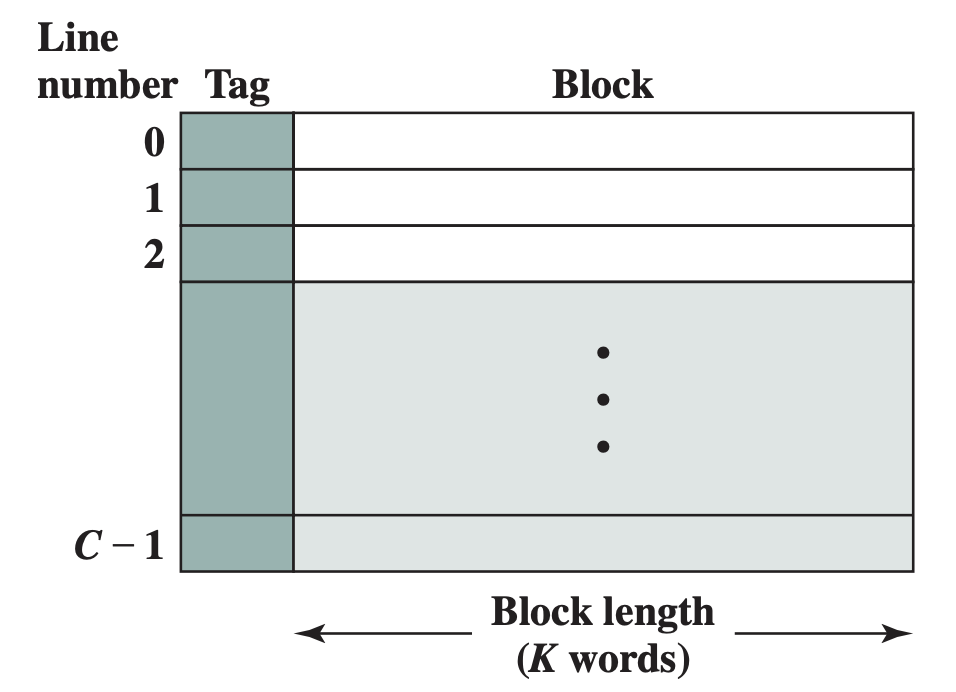
\includegraphics[width=0.4\linewidth]{chaps/memory/cache-memory/cache-mem-organisation.png}
\caption{Cache Memory Organisation}
\end{figure}

\subsubsection{Cache Memory Read}

The process of reading from the cache is roughly described as follows:
\begin{enumerate}
    \item Obtain the address of the word to be read from the CPU.
    \item Check if the block containing the word is in the cache.
    \begin{enumerate}
        \item If the block is in the cache, read the word from the cache.
        \item If the block is not in the cache, load the block from the main memory
            into the cache, and \textbf{at the same time} deliver the word to the CPU.
    \end{enumerate}
\end{enumerate}

\subsubsection{Address Mapping}

There are three ways to map the main memory to the cache:
\begin{enumerate}
\item \textbf{Direct Mapping}: 
    Each block of main memory maps to exactly one line in the cache. The mapping is
    given as $i = j \bmod m$, where $i$ is the cache line number, $j$ is the main memory
    block number, and $m$ is the number of cache lines.
    
    \begin{example}
        The cache logic treats the main memory address in three parts as follows:
        \begin{equation*}
            \underbrace{0000\,0001}_{(s-r)\text{ bits (tag)}}\,
            \overbrace{1111\,1111\,1111\,11}^{r\text{ bits (line number)}}
            \underbrace{00}_{w\text{ bits (word)}}
        \end{equation*}
        The least significant $w$ bits identify the word within the block,
        where the block size is $2^w$ words. The next $r$ bits identify the line
        number within the cache memory, where the cache memory has $2^r$ lines.
        The most significant $(s-r)$ bits are the tag bits, which are used to
        distinguish between the different main memory blocks that map to the same line,
        where the main memory has $2^s$ blocks.
    \end{example}

    To perform a read operation, the line number first identifies the line in the cache.
    Then, the tag bits in the line are compared with the tag bits in the address.
    If the tags match, the word is read from the cache according to the word bits in the
    address. If the tags do not match, the block is read from the main memory into the
    cache, and the word is read from the cache.

    \begin{multicols*}{2}
        \textbf{Advantages}: \begin{itemize}
            \item Only need to check one cache line, fast.
            \item No selection is required, less use of logic gates, inexpensive.
        \end{itemize}
        \columnbreak
        \textbf{Disadvantages}: \begin{itemize}
            \item When two blocks map to the same line are accessed alternatively,
                constant cache misses occur.
            \item The cache is not fully utilised.
        \end{itemize}
    \end{multicols*}

\item \textbf{Fully Associative Mapping}:
    Any block of main memory can be loaded into any line of the cache. The main memory
    address is treated as two parts only -- the tag and the word bits. Again, for a main
    memory address of $(s+w)$ bits, and a cache memory with block length of $2^w$ words,
    the word bits are the least significant $w$ bits, and the tag bits are the remaining
    $s$ bits.

    To perform a read operation, the cache controller searches the entire cache for the
    desired tag. If it is a miss, the block is read from the main memory into the cache.

    \begin{multicols}{2}
        \textbf{Advantages}: \begin{itemize}
            \item More flexible use of cache than direct mapping.
        \end{itemize}
        \columnbreak
        \textbf{Disadvantages}: \begin{itemize}
            \item Requires more complex logic and circuits for tag comparison, more expensive.
            \item Must simultaneously search all cache lines, slower.
        \end{itemize}
    \end{multicols}

\item \textbf{Set Associative Mapping}:
    The cache consists of a number of sets, and each sets consists of a number of lines.
    Their relationship is given by
    \begin{align*}
        m &= v \times k \\
        i &= j \bmod v
    \end{align*}
    where $i$ is the set number, $j$ is the main memory block number, $m$ is the number
    of lines in cache, $v$ is the number of sets, and $k$ is the number of lines in each set.
    ($k$ is usually 2, the maximum is 8.) Also referred to as $k$-way set associative mapping.

    Block $B_j$ in main memory maps to any of the lines in set $j$ in the cache. There are
    two ways of implementing a set associative mapping, either as
    \begin{enumerate}
        \item $v$ assiciative-mapped caches 
            (usually used for high associativity, i.e. larger $k$).
            Each cache is called a \textbf{set}.
        \item $k$ direct-mapped caches (for lower associativity).
            Each cache is called a \textbf{way}.
    \end{enumerate}

    The cache control logic treats the $(s+w)$-bit main memory address in three parts:
    tag, set, and word.
    The $d$ bits of set identifies the set in cache, where $v = 2^d$.
    The least significant $w$ bits identify the word.
    The remaining $(s-d)$ bits are the tag bits.

    With this method, the tag size is much smaller than in fully associative mapping,
    and each tag is only compared with $k$ tags in a single set.

    \begin{multicols}{2}
        \textbf{Advantages}: \begin{itemize}
            \item Fewer misses than direct mapping.
        \end{itemize}
        \columnbreak
        \textbf{Disadvantages}: \begin{itemize}
            \item Complex selection and comparison logic, slightly slower.
        \end{itemize}
    \end{multicols}

\end{enumerate}